\chapter{Analisi handshake TLS}
I livelli analizzati in precedenza consentono una corretta comunicazione, ignorando però aspetti importanti quali confidenzialità, integrità ed autenticità; vi è quindi il bisogno di estendere lo stack introducendo un nuovo layer, facoltativo, in grado di garantire queste caratteristiche.
Questo livello viene posizionato tra quello di trasporto e quello applicativo. 

\begin{table}[h]
	\centering
	\begin{tabular}{| l | c |}
		\hline
		Livello 7 & Applicativo
		\\
		\hline
		\rowcolor{yellow!10}Livello 5 & Sicurezza
		\\
		\hline
		Livello 4 & Trasporto
		\\
		\hline
		Livello 3 & Rete
		\\
		\hline
		Livello 2 & Fisico
		\\
		\hline
		
	\end{tabular}
	\caption{Livelli dello stack con layer di sicurezza}
	\label{tab:stackTLS}
\end{table}

Per garantire la confidenzialità dei dati in rete, ovvero la loro segretezza, si fa uso della crittografia ovvero una procedura che modifica i pacchetti in modo da renderli incomprensibili ad attori esterni alla comunicazione.
Questa avviene solitamente in forma simmetrica, ovvero la chiave per cifrare i dati è la medesima utilizzata per decifrarli.

\section{Handshake TLS}
La presenza di una chiave comune ad entrambi i partecipanti della comunicazione pone il problema di come questi ne vengano a conoscenza, non potendosi effettuare lo scambio di chiavi sul medesimo canale delle comunicazioni ordinarie in quanto insicuro.
Oltre alla confidenzialità della chiave, si ha inoltre il problema dovuto all'autenticità della stessa; un eventuale attaccante potrebbe infatti intromettersi nella comunicazione prendendo il posto di uno dei due host, all'insaputa dell'altro (attacco Man In The Middle, MITM).

TLS è un protocollo che prevede uno scambio di messaggi precedente all'invio dei dati veri e propri (handshake) che permette una successiva comunicazione sicura. Si precisa che i pacchetti inviati a questo scopo non sono cifrati, non essendoci ancora una chiave di cifratura in possesso degli host. Solo al termine di questa procedura si saranno scambiate correttamente le chiavi.

Il primo messaggio è inviato dal client al server e prende il nome di \textit{client hello}. In questo messaggio vengono inviate informazioni quali cifrari supportati (in ordine di preferenza), versione TLS in uso, ed estensioni che specificano altri aspetti come ad esempio il supporto alle curve ellittiche o a determinati algoritmi di hashing per il controllo dell'autenticità.

Il server risponde indicando il cifrario da utilizzare, le estensioni da lui supportate, il suo certificato (per garantire l'autenticità della risposta) oltre ad iniziare lo scambio di chiavi, effettuato sfruttando meccanismi matematici in grado di garantire la confidenzialità di quest'ultima anche in caso di MITM passivo.
A questo punto il client termina lo scambio di chiavi.

\section{Browser fingerprinting}
L'analisi delle differenze nel contenuto dei pacchetti client hello inviati da differenti client permette di notare differenze peculiari di quest'ultimi, consentendone la sua individuazione; in questo documento saranno analizzati i browser più popolari.
\\

I browser analizzati sono stati i seguenti:
\begin{itemize}
	\item Chrome versione 105.0.5195.127
	\item Mozilla Firefox versione 105.0
	\item Microsoft Edge versione 105.0.1343.42
	\item Opera versione 91.0.4516.20
\end{itemize}
Non è stato preso in considerazione Safari, in quanto non vi è una versione aggiornata per Windows.
\\

Nel processo di analisi sono stati ispezionati i cifrari utilizzati, l'utilizzo del GREASE, gli algoritmi di hashing supportati e altre estensioni come ad esempio il supporto alle curve ellittiche.

Esaminando i cifrari supportati, si può notare la loro differenza in numero:
\\
\begin{table}[h]
	\centering
	\begin{tabular}{| l | c |}
		\hline
		\rowcolor{yellow!10}Chrome & 16
		\\
		\hline
		\rowcolor{orange!10}Firefox & 17
		\\
		\hline
		\rowcolor{blue!10}Edge & 17
		\\
		\hline
		\rowcolor{red!10}Opera & 16
		\\
		\hline
		
	\end{tabular}
	\caption{Cifrari supportati dai vari browser}
	\label{tab:cifrari}
\end{table}
Questo rende Edge e Firefox differenti rispetto agli altri due, in quanto supportano un numero di cifrari diverso. Firefox, però, presenta anche altre differenze rispetto agli altri come per esempio il supporto ad un maggior numero di algoritmi di hashing e la non presenza del GREASE nei cifrari. 
Per quanto riguarda il primo valore, Firefox è l'unico a presentare un numero diverso rispetto agli altri:

\begin{table}[H]
	\centering
	\begin{tabular}{| l | c |}
		\hline
		\rowcolor{yellow!10}Chrome & 8
		\\
		\hline
		\rowcolor{orange!10}Firefox & 11
		\\
		\hline
		\rowcolor{blue!10}Edge & 8
		\\
		\hline
		\rowcolor{red!10}Opera & 8
		\\
		\hline
		
	\end{tabular}
	\caption{Algoritmi di hashing supportati}
	\label{tab:hash}
\end{table}

Il GREASE,  acroninimo di Generate Random Extensions And Sustain Extensibility, è un valore che corrisponde ad un cifrario inesistente nella realtà e che quindi il ricevente deve ignorare; il protocollo prevede infatti che se il server non supporta un cifrario nella lista questo vada ignorando, valutando quello successivo. Si tratta perciò di un test utile per prevenire bug.
È quindi logico che il GREASE venga posizionato in cima alla lista dei cifrari, in modo che sia sempre valutata dal server.
\\
Anche in questo caso, Firefox è l'unico browser a comportarsi differentemente rispetto agli altri:
\\
\begin{table}[h]
	\centering
	\begin{tabular}{| l | c |}
		\hline
		\rowcolor{yellow!10}Chrome & Sì
		\\
		\hline
		\rowcolor{orange!10}Firefox & No
		\\
		\hline
		\rowcolor{blue!10}Edge &Sì
		\\
		\hline
		\rowcolor{red!10}Opera & Sì
		\\
		\hline
		
	\end{tabular}
	\caption{Presenza del GREASE nella lista dei cifrari supportati}
	\label{tab:grease}
\end{table}

Analizzando nel dettaglio il client hello inviato da Edge, si può notare una caratteristica piuttosto peculiare. Vi è infatti un cifrario, per l'esattezza il \textbf{AES 256 GCM SHA384}, che viene ripetuto due volte all'interno della lista dei cifrari. Questo è ovviamente inutile, in quanto se il server rifiuta quest'ultimo poi procederebbe a valutarlo nuovamente, producendo quindi un nuovo rifiuto. Si tratta dell'unico browser dei quattro che ha questo comportamento, che lo rende molto vulnerabile al fingerprinting.
Di seguito lo screenshot di Wireshark che mostra questa caratteristica.

\begin{figure}[h]
	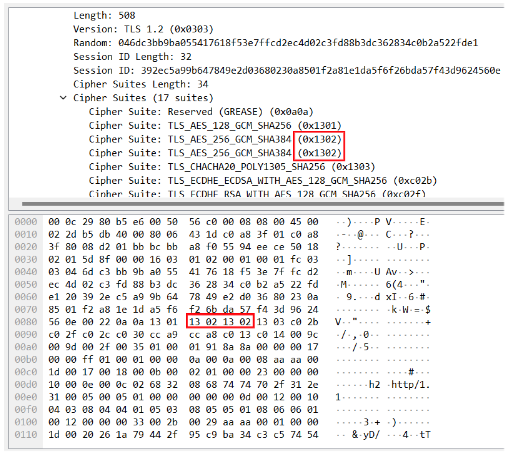
\includegraphics[width=\textwidth]{figures/cifrario_ripetuto.png}
	\caption{Pacchetto client hello inviato tramite Microsoft Edge}
	\label{cifrario_ripetuto}
\end{figure}

Questo causa una differenza di comportamento tra Chrome e Firefox, agevolando il loro riconoscimento. Eliminare il cifrario ripetuto porterebbe Edge ad una situazione uguale a quella di Chrome e Opera, rendendoli quindi indistinguibili.



 








